\documentclass[11pt, oneside]{article} 
\usepackage{geometry}
\geometry{letterpaper} 
\usepackage{graphicx}
	
\usepackage{amssymb}
\usepackage{amsmath}
\usepackage{parskip}
\usepackage{color}
\usepackage{hyperref}

\graphicspath{{/Users/telliott_admin/Tex/png/}}
% \begin{center} 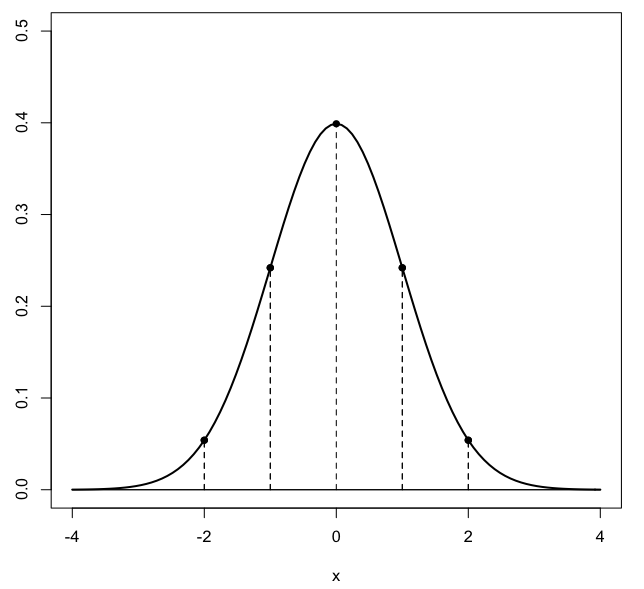
\includegraphics [scale=0.4] {gauss3.png} \end{center}

\title{Sums of integers}
\date{}

\begin{document}
\maketitle
\large

In what follows we are looking for simple formulas to calculate the value of expressions of the form
\[ \sum_{k=1}^{n} f(k) \]
For simplicity we suppress the indices and write
\[ \sum f(k) \]

\subsection*{sum of integers}
The first example is a formula for the sum of the integers $1 \dots n$ = $\sum k$.  

There's a trick!  Write:
\[ \sum (k + 1)^2 = \sum \ [ \ k^2 + 2k + 1 \ ] \]
A fundamental rule for sums is that they can be broken up (by associativity):
\[ \sum (k + 1)^2 = \sum k^2 + \sum 2k + \sum 1 \]
\subsection*{telescoping sum}

Now, move the first term on the right-hand side over to the left and consider:
\[ \sum (k + 1)^2 - \sum k^2 \]
Write out the individual terms of each sum
\newpage

\[ \hspace{30mm}  = [ \ 2^2 + 3^2 + \dots + n^2 + (n+1)^2 \ ] \]
\[ - \ [ \ 1^2 + 2^2 + 3^2 + \dots + n^2 \ ] \]
Every term in the first set of brackets has a counterpart in the second one to cancel it, except $(n+1)^2$.  Similarly, every term in the second part except $1^2$ cancels.

So the end result is
\[ = (n+1)^2 - 1 \]
And after expanding the square we can cancel the $1$
\[ = n^2 + 2n \]
This is called a \emph{telescoping} sum.
\subsection*{algebra}
We now have
\[ n^2 + 2n = \sum 2k + \sum 1 \]
Factor out the $2$
\[ n^2 + 2n = 2 \sum k + \sum 1 \]
$\sum k$ is what we seek.  The other term is
\[ \sum 1 = 1 + 1 + \dots + 1 \]
In the sum on the right there are $n$ terms, so $\sum 1 = n$
\[ n^2 + 2n = 2 \sum k + n \]
\[ \frac{n^2 + n}{2} = \sum k \]
\[ \sum k = \frac{n(n+1)}{2} \]
A familiar result.
\begin{center} 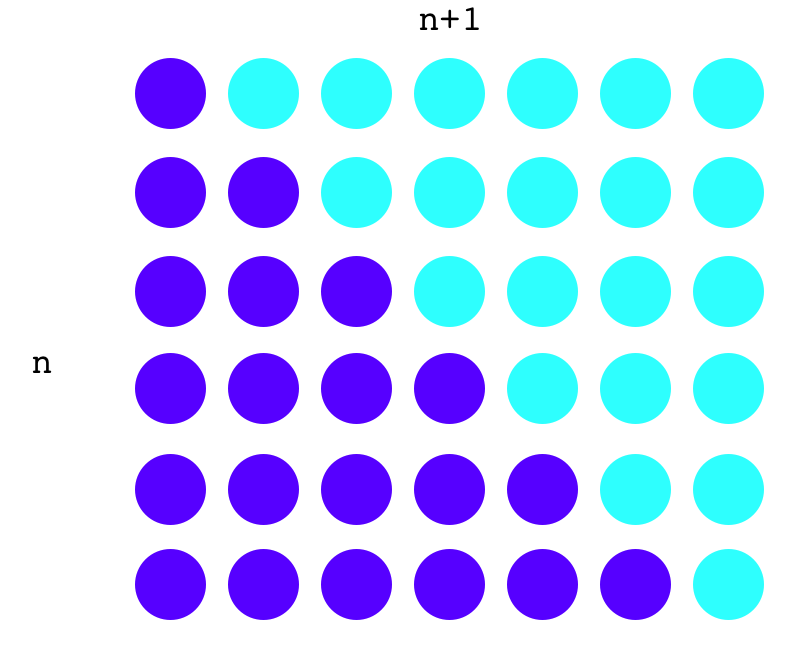
\includegraphics [scale=0.15] {sum_n.png}\end{center}

\subsection*{sum of integers, squared}
Write:
\[ \sum (k + 1)^3 = \sum \ [ \ k^3 + 3k^2 + 3k + 1 \ ] \]
Move the first term on the right to the left-hand side, and we have another telescoping sum, which after the subtraction, gives us
\[ (n + 1)^3 - 1 = \sum 3k^2 + \sum 3k + \sum 1 \]
Factor out the $3$
\[ (n + 1)^3 - 1 = 3 \sum k^2 + 3 \sum k + \sum 1 \]
$\sum k^2$ is what we seek.  

$\sum k$ is what we obtained in the previous section and $\sum 1 = n$, as before:
\[ (n + 1)^3 - 1 = 3 \sum k^2 + \frac{3n(n+1)}{2} + n \]
\subsection*{algebra}
Expand the left-hand side and cancel the $\pm 1$
\[ n^3 + 3n^2 + 3n = 3 \sum k^2 + \frac{3n(n+1)}{2} + n \]
Multiply by $2$
\[ 2n^3 + 6n^2 + 6n = 6 \sum k^2 + 3n(n+1) + 2n \]
\[ 2n^3 + 3n^2 + n = 6 \sum k^2  \]
\[ n(2n^2 + 3n + 1) = 6 \sum k^2  \]
\[ n(n + 1)(2n + 1) = 6 \sum k^2  \]
\[  \sum k^2 = \frac{n(n + 1)(2n + 1)}{6} \]
\[ = \frac{n(n+1)}{2} \cdot \frac{(2n+1)}{3} \]

\subsection*{sum of integers, cubed}
Write:
\[ \sum (k + 1)^4 = \sum \ [ \ k^4 + 4k^3 + 6k^2 + 4k + 1 \ ] \]
\[ \sum (k + 1)^4 = \sum k^4 + \sum 4k^3 + \sum 6k^2 + \sum 4k + \sum 1 \ ] \]
Move the first term on the right to the left-hand side, and we have another telescoping sum, which after the subtraction, gives us
\[ (n + 1)^4 - 1 = 4 \sum k^3 + 6 \sum k^2 + 4 \sum k + \sum 1 \] 

First, expand the left-hand side and cancel the $1$'s:
\[ n^4 + 4n^3 + 6n^2 + 4n =  4 \sum k^3 + 6 \sum k^2 + 4 \sum k + \sum 1 \]
$\sum k^3$ is what we seek. 

We have previously derived expressions for the other sums, so substitute them
\[ n^4 + 4n^3 + 6n^2 + 4n =  4 \sum k^3 + 6 \ [ \frac{n(n + 1)(2n+1)}{6} \ ] \ + 4 \ [ \ \frac{n(n + 1)}{2}  \ ] \ + n \]
Reduce the fractions
\[ n^4 + 4n^3 + 6n^2 + 4n =  4 \sum k^3 + n(n + 1)(2n+1) + 2 n(n + 1) + n \]
Cancel the solitary $n$
\[ n^4 + 4n^3 + 6n^2 + 3n =  4 \sum k^3 + n(n + 1)(2n+1) + 2 n(n + 1)  \]
At this point we could multiply out the right-hand side and cancel some terms, but notice that we can factor the left-hand side, finding just an $n$ but also an $(n+1)$:
\[ n(n^3 + 4n^2 + 6n + 3) =  4 \sum k^3 + n(n + 1)(2n+1) + 2 n(n + 1)  \]
\[ n(n+1)(n^2 + 3n + 3) =  4 \sum k^3 + n(n + 1)(2n+1) + 2 n(n + 1)  \]
So then, gathering terms 
\[ 4 \sum k^3 = n(n+1) \ [ \ n^2 + 3n + 3 - 2n - 1 - 2 \ ]  \]
\[ = n(n+1) \ [ \ n^2 + n \ ]  \]
\[ \sum k^3 = \frac{n(n+1)}{2} \ \frac{n(n+1)}{2} \]

\subsection*{induction}
We check the first formula
\[ \sum_{k=1}^n k = \frac{n(n+1)}{2} \]
by using induction to prove it.
 
The base case is $1 = 1(1 + 1)/2 = 1$.  Good.  Then we must show that
\[ \sum_{k=1}^{n+1} k = \sum_{k=1}^{n} k + (n + 1) \]
\[ = \frac{(n)(n+1)}{2} + (n + 1) \]
\[ = \frac{(n)(n+1)}{2} + \frac{2(n + 1)}{2} \]
\[ = \frac{(n+1)(n+2)}{2}  \]

which is exactly what we get by substituting $(n+1)$ for $n$ in the formula
\[ \sum_{k=1}^n k = \frac{n(n+1)}{2} \]
\[ \sum_{k=1}^{n+1} k = \frac{(n+1)(n+2)}{2} \]

\subsection*{sum of integers, to the fourth power}

One last time.
The first expression looks pretty forbidding, a quintic:
\[ \sum (k + 1)^5 = \sum \ [ \ k^5 + 5k^4 + 10k^3 + 10k^2 + 5k + 1 \ ] \]
Similar to what we did before,
\[ \sum (k + 1)^5- \sum k^5 = (n+1)^5 - 1 \]
On the right-hand side we have $5 \sum k^4$ which what we seek, and then
\[ 10 \sum k^3 + 10 \sum k^2 + 5 \sum k + \sum 1 \]
\[ =  10 \ [ \ \frac{n(n+1)}{2} \ \frac{n(n+1)}{2} \ ] \ + 10 \ [ \ \frac{n(n+1)}{2} \cdot \frac{(2n+1)}{3}  \ ] + 5 \ [ \ \frac{n(n+1)}{2} \ ] \ + n \ \]

That looks like a mess, but let's move the trailing $n$ to the left-hand side and then see if we can find a factor of $n(n+1)$ on the left, just like before:
\[ (n+1)^5 - 1 - n \]
\[ = n^5 + 5n^4 + 10n^3 + 10n^2 + 4n \]
Obviously, we have a factor of $n$
\[ = n (n^4 + 5n^3 + 10n^2 + 10n + 4) \]
And just on faith, I know we can find a factor of $(n+1)$ as well:
\[ = n (n+1) (n^3 + 4n^2 + 6n + 4) \]
You'll see it checks if you multiply out.

So now we write out the whole thing 
\[ 5 \sum k^4 = n (n+1) \ [ \ (n^3 + 4n^2 + 6n + 4) - \frac{10}{4} \ n (n+1) - \frac{10}{6} \  (2n + 1) - \frac{5}{2}  \ ] \]

Multiply both sides by $6$ and reduce the fractions
\[  30 \sum k^4 = n (n+1) \ [ \ (6 n^3 + 24 n^2 + 36n + 24) - 15 n (n+1) - 10  (2n + 1) - 15  \ ] \]
Let's try to work with what's in the brackets on the right
\[  6n^3 + 24n^2 + 36n + 24 - 15 n^2 - 15n - 20n -10 - 15 \]
\[  6 n^3 + 9 n^2 + 11 n - 1  \]
I don't think that can be factored with integers.
\[  30 \sum k^4 = n (n+1) \ [ \ 6 n^3 + 9 n^2 + 11 n - 1 \ ]  \]

\end{document} 